% !TEX root = ../MasterThesis.tex
\chapter{Refutation}
\label{chap:refutation}

Refutation is the search for a counterexample that invalidates a candidate certificate. The counterexample is an explicit state in the sense of Definition~\ref{def:verification} --- one violating the condition of interest --- which we then use to guide the next round of CEGIS. Counterexamples are much easier to find than proofs of their absence, primarily because the claim changes shape: instead of establishing the condition for \emph{all} $x \in \aX$, it suffices to exhibit \emph{some} $x \in \aX$ that violates it. This lets us treat the problem as a search, which careful formulation can pose in several efficient ways. In this chapter we benchmark six black-box optimisers, testing them on standard test problems as well as real neural certificates to assess their usefulness as a dedicated subroutine in the CEGIS pipeline.


Let 
\[
x^\star = \argmax_{x \in \aX} \drift(x).
\]
From an optimisation perspective, verification checks
\[
\drift(x^\star) \leq 0,
\]
whereas any $x \in \aX$ such that
\[
\drift(x) > 0
\]
is in fact a counterexample. Whilst all the aforementioned verification methods can find these counterexamples and serve as refuters, we can also consider specialised refuters that are designed around this optimisation problem.

\section{Optimisers}

Optimisers are an attractive choice for refutation for two reasons. First, global optimisation is a mature field, so there is a large body of prior research to draw well-performing optimisers from. Second, optimisers are readily customised: the objective function, constraints, and search targets can each encode whatever information our assumptions permit, steering the search accordingly.

As this is for refutation and not for verification, strict soundness is no longer of concern, and even points that seem close to counterexamples provide insight into the margin we have certified for. This makes a Monte-Carlo approximation of the expectation good enough for our use case. For each point evaluation, we take $m$ Monte-Carlo samples of the successor state, resulting in the objective function $\tilde{\drift}(x) = \frac{1}{m} \sum_{i=1}^{m} \cert(f(x, w_i)) - \cert(x) + \varepsilon$. Occasionally this can cause spurious counterexamples, leading to bad early-termination or incorrect local maxima.


\subsection{Random Search}

Random search is the most naive method of search in which we take uniform, iid samples across $\aX$, tracking only the best evaluations and disregarding the rest. It is simple to implement, extremely fast, but completely uninformed. It effectively acts as a benchmark for counterexample quality: the larger the drift value, the larger the violation, and the better the quality of the counterexample.

\subsection{Grid Search}

Grid search is analogous to a non-adaptive MAB algorithm. We grid the domain and evaluate centres, then refine and repeat uniformly across the domain. As a result, it is often centred on the domain and takes symmetrical evaluations which can sometimes be beneficial and other times wasteful. With each iteration the number of points to evaluate grows exponentially, so its per-iteration cost climbs with the point count. Both grid search and random search are everywhere-dense in the limit of infinite resources.


\subsection{DIRECT}

DIRECT (DIviding RECTangles) \cite{Jones1993DIRECT} reframes global optimisation as a recursive partition of the search domain into hyper-rectangles, each represented by its centre. At each iteration it identifies the potentially optimal rectangles, balancing exploitation of regions with high centre values against exploration of large, under-sampled regions. Unlike traditional Lipschitz optimisation methods, DIRECT does not require a user-specified Lipschitz constant; instead, it implicitly considers all possible positive Lipschitz constants when selecting rectangles for refinement. The selected rectangles are trisected along their longest dimension(s), and the centres of the resulting subrectangles are evaluated. Because the selection rule simultaneously considers rectangles across multiple scales, DIRECT naturally balances local refinement with global exploration and rarely commits prematurely to a single basin. Aside from a small parameter $\varepsilon_{\mathrm{po}}$ used to avoid excessive refinement of the current best region, the method is effectively parameter-free. Its main computational cost lies in maintaining the growing set of rectangles and identifying the potentially optimal subset via a convex-hull computation.

\subsection{AdaLIPO}

AdaLIPO (Adaptive Lipschitz Optimisation) \cite{malherbe2017global} is a purely sample-driven Lipschitz
method. It keeps a history of evaluated points, and each iteration proposes a
large uniform pool of candidates, scoring each by the tightest upper bound its
history allows, $\min_i [\, y_i + \hat{k}\,\lVert x - x_i\rVert \,]$, and spends
its evaluation budget on the most promising ones. The Lipschitz constant
$\hat{k}$ is estimated online from the steepest slope seen so far and inflated
slightly to stay optimistic. This makes AdaLIPO a natural fit for refutation: it
exploits precisely the regularity we already assume of the drift --- its
Lipschitz continuity --- to steer samples toward the region most likely to hide
a violation, rather than searching blindly. The overhead is the pairwise
distance computation against the history, which grows with the number of
evaluations.

\subsection{Hill Climbing (HC)}

HC exploits differentiability to traverse the landscape, wherein an agent explores in the direction that the derivative is most positive. It is the counterpart to Gradient Descent, which is famously used in machine learning for minimising loss functions. In its most basic form, it is susceptible to getting stuck at local maxima, and as such we employ random restarts to encourage the agent to explore more of the state space. Because JAX provides automatic differentiation and JIT compilation, we run HC efficiently on GPU and vectorise it so that many restarts search at once. Crucially, this gradient access is an extra assumption made only by HC.

\subsection{Whale Optimisation Algorithm (WOA)}

WOA \cite{whale_oa} is a population-based metaheuristic inspired by the bubble-net hunting of
humpback whales. A population of candidate points moves each iteration by one of
three behaviours relative to the incumbent best: a shrinking \emph{encircle}, a
logarithmic \emph{spiral}, or an \emph{exploratory} step toward a random peer. A single parameter $a$ anneals
linearly over the budget, shifting the population from exploration to
exploitation. The spiral gives WOA a distinctive ability to probe around a
promising point at many radii at once, and being population-based it is
naturally parallel and resistant to being trapped by a single local optimum. It
also carries the most tuning knobs of the refuters we consider: the annealing
ceiling $a_{\max}$, the spiral tightness $b$, and the spiral/encircle mix $p$.
Crucially, WOA has a track record as a fast and flexible black-box optimiser,
performing consistently in optimiser comparisons on the Black-Box Optimisation
Benchmarking (BBOB) suite of the COCO platform \cite{hansen2021coco}.

\section{Experiments}

We study the refuters in two stages. Because they cannot certify on their own,
their value in the pipeline is as a cheap pre-screen: run up to a fixed budget
each round, falling back on the sound verifier only when no counterexample is
found --- the arrangement Chapter~\ref{chap:streamlining} evaluates
end-to-end. We first tune each refuter as a black-box optimiser on a standard benchmark suite
(Section~\ref{sec:bbob}), then turn the tuned refuters on genuine refutation
tasks (Section~\ref{sec:fauxcert}).

\subsection{Hyperparameter Tuning on BBOB}
\label{sec:bbob}

Before comparing refuters we must give each a fair chance, which means choosing
its hyperparameters well. We take five functions from the BBOB test suite, spanning
the landscape archetypes that separate search strategies: Rastrigin (f3, a
regular grid of local optima), Rosenbrock (f8, a narrow curved valley),
Schaffers~F7 (f17, irregular ripples at every radius), Schwefel (f20, best basins are far from the centre), and
Gallagher's 101-peak function (f21, a narrow needle among distractors). Each is
negated so that the refuter \emph{maximises} and the global optimum is $0$; every
function is first checked for well-formedness (Figure~\ref{fig:bbob-landscapes}).




\begin{figure}[htbp]
\centering
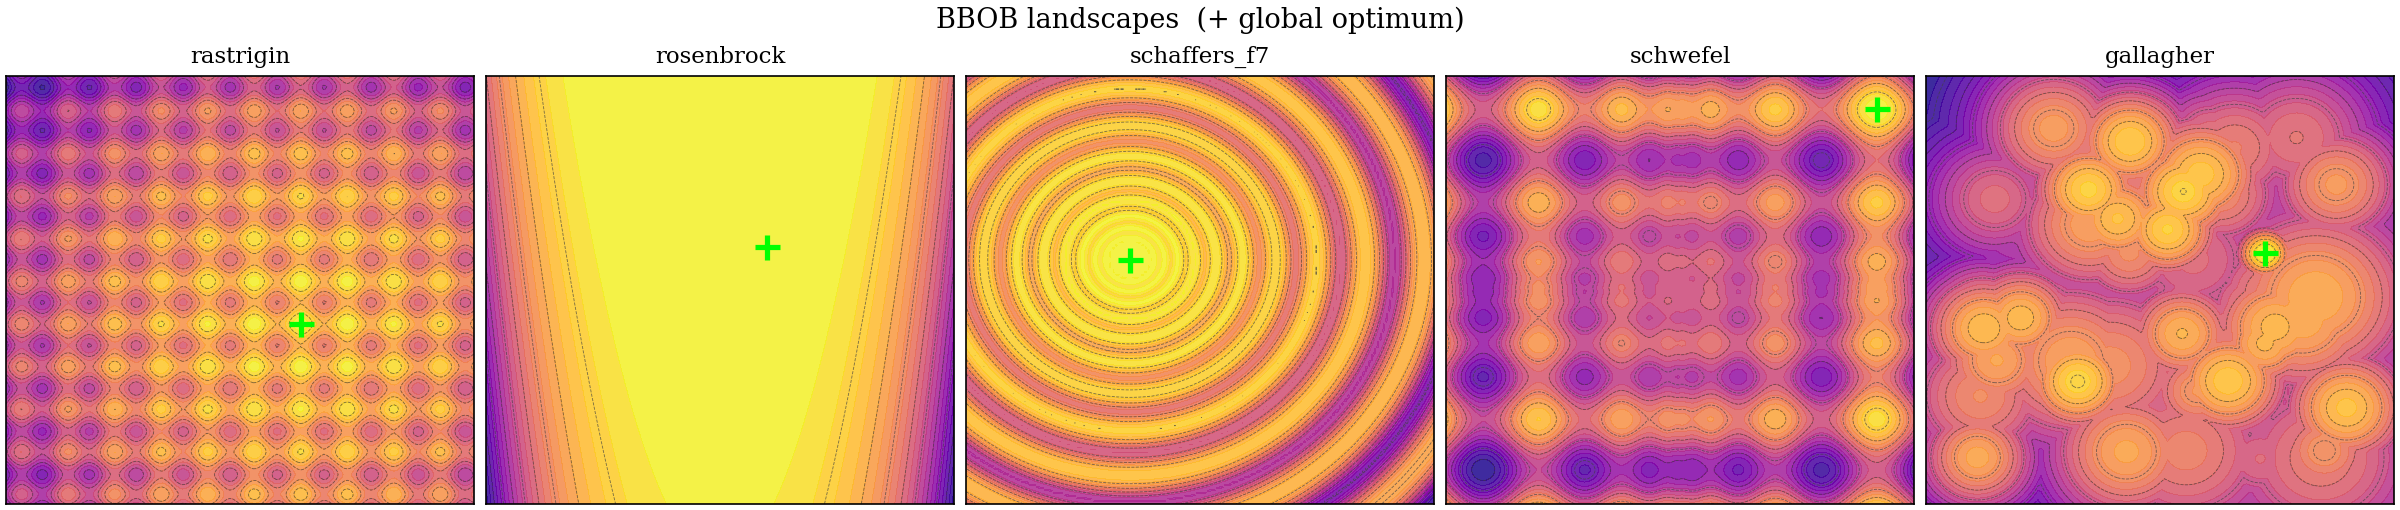
\includegraphics[width=\linewidth]{Figures/bbob_landscapes.png}
\caption{The five BBOB test functions with the
global optimum marked in green. Yellow indicates high-quality solutions and purple indicates low-quality solutions.}
\label{fig:bbob-landscapes}
\end{figure}

For each refuter we sweep its hyperparameter grid over the five functions and
three seeds at a budget of $8192$ evaluations, and score a run by its
\emph{normalised regret} $r = -\,\hat{y}^\star / \mathrm{Diam}(f) \in [0,1]$,
where $\hat{y}^\star$ is the best value found and $\mathrm{Diam}(f)$ the span of
$f$ over the domain, so that $r=0$ means the optimum was located. The best
hyperparameters for a refuter are those minimising the mean regret over
functions and seeds; Table~\ref{tab:bbob-best} reports them.

\begin{table}[htbp]
\centering
\begin{tabular}{llrr}
\hline
Refuter & Best hyperparameters & Mean regret & Time (s) \\
\hline
Whale (WOA)   & $a_{\max}=1.5,\ b=0.5,\ p=0.75$     & $5.8\times10^{-8}$ & $0.004$ \\
DIRECT        & $\varepsilon_{\mathrm{po}}=10^{-3}$ & $3.7\times10^{-5}$ & $0.148$ \\
AdaLIPO       & $\text{pool}=16,\ \alpha=0.2$       & $4.9\times10^{-4}$ & $0.686$ \\
Grid          & ---                                 & $2.3\times10^{-3}$ & $0.001$ \\
Random        & ---                                 & $5.1\times10^{-3}$ & $0.002$ \\
Hill climbing & $\text{lr}=0.5,\ \text{decay}=0.95$ & $5.7\times10^{-3}$ & $0.002$ \\
\hline
\end{tabular}
\caption{Best hyperparameters per refuter, by mean normalised regret over the
five BBOB functions and three seeds. Lower regret is
better; time is the mean wall-clock per search.}
\label{tab:bbob-best}
\end{table}

Two results stand out. First, the Lipschitz-aware and population methods
dominate the uninformed ones: whale, DIRECT and AdaLIPO reach regrets one to
five orders of magnitude below random, grid and hill climbing. Second,
accuracy need not be bought with time: whale in particular solves all five
landscapes at essentially zero regret in milliseconds, a combination that
Figure~\ref{fig:bbob-time} places on the quality--cost plane below.


Figure~\ref{fig:bbob-quality} breaks the tuned refuters down by function.
Rosenbrock's valley is easy for everyone at this budget; it is the multimodal
and deceptive functions that separate the methods. Hill climbing is competitive
only on the smooth valley and the ripples, and collapses on Schwefel (two orders
of magnitude worse than plain grid search) and Gallagher which punish pure exploitation.
 Whale and DIRECT solve every function; AdaLIPO
is a consistent middle tier. Figure~\ref{fig:refuter-patterns} shows how the refuters differ in where they
spend their evaluations on a shared landscape, from the uniform scatter of
random search to the basin-focused trajectories of the informed methods.


\begin{figure}[htbp]
\centering
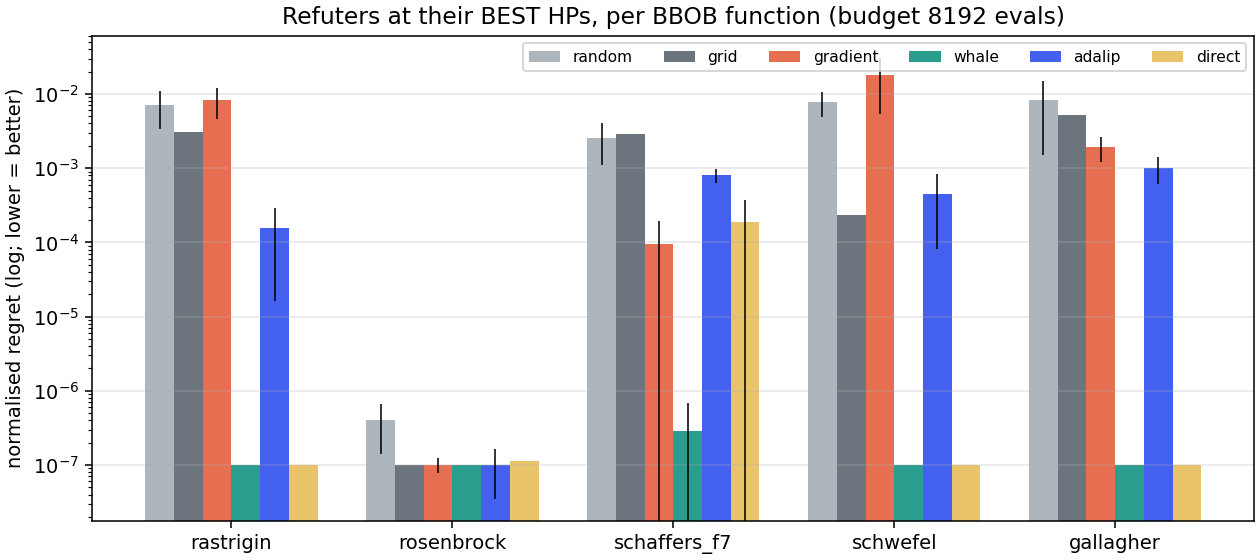
\includegraphics[width=\linewidth]{Figures/bbob_quality_per_function.png}
\caption{Normalised regret (log scale) of each refuter at its best
hyperparameters, per BBOB function. The multimodal and deceptive functions
(Schwefel, Gallagher, Rastrigin) separate the informed methods from the
uninformed ones.}
\label{fig:bbob-quality}
\end{figure}

Finally, Figure~\ref{fig:bbob-time} places quality against wall-clock cost. Two
clusters emerge: a fast-and-accurate frontier occupied by whale (millisecond
searches at essentially zero regret) and a slower, deliberate cluster (AdaLIPO
and DIRECT at tenths of a second, paying their per-iteration Lipschitz
bookkeeping for accuracy). Random, grid and hill climbing are fast but sit three
to five orders of magnitude worse on the hard functions. Whale at its tuned
configuration dominates the frontier outright, and it is these tuned
configurations that we carry into the refutation experiment that follows.

\begin{figure}[htbp]
\centering
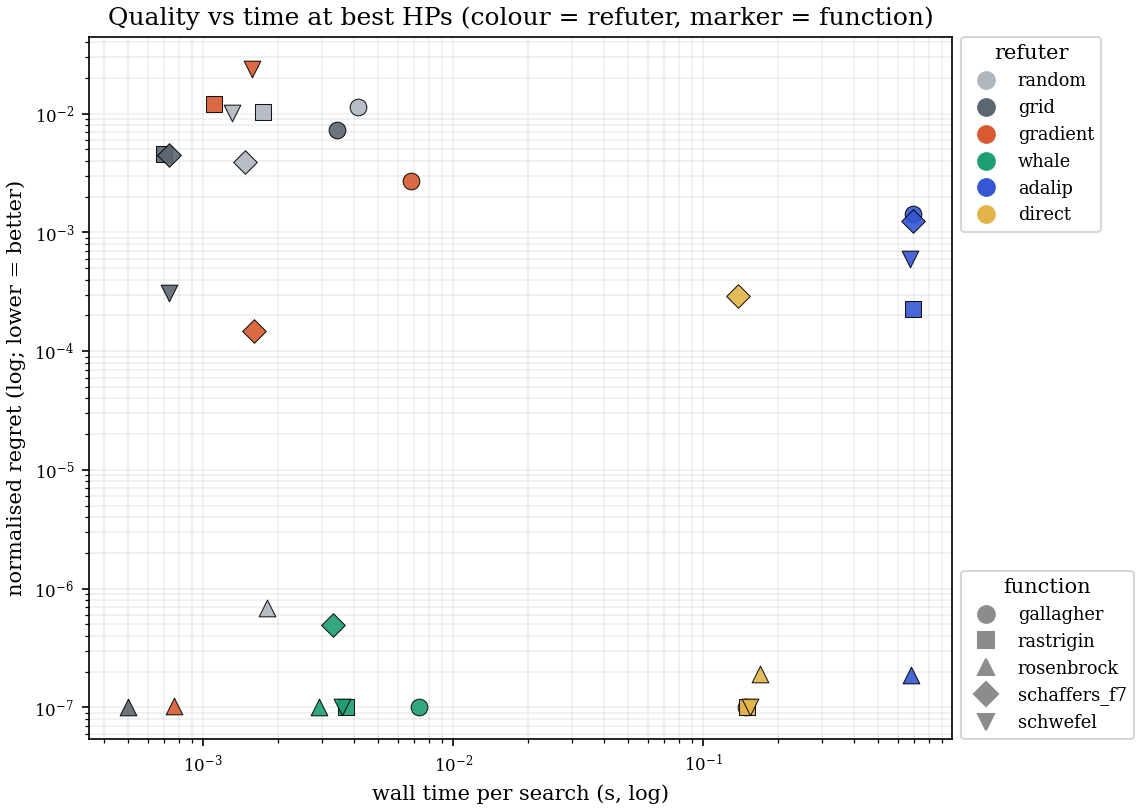
\includegraphics[width=0.8\linewidth]{Figures/bbob_quality_vs_time.png}
\caption{Quality versus wall-clock cost at the best hyperparameters (colour =
refuter, marker = function; both axes logarithmic). Whale occupies the
fast-and-accurate frontier; the Lipschitz methods trade time for accuracy;
uninformed search is fast but far worse on the hard landscapes.}
\label{fig:bbob-time}
\end{figure}

\subsection{Refuting Faux Certificates}
\label{sec:fauxcert}

The BBOB benchmark tunes and characterises the refuters as generic optimisers;
we now experiment with refuters within the context of our problem definition. Every round in
which a sound verifier (MILP or LiRPA) rejected a candidate certificate during
the verification runs of the previous chapter left behind a \emph{faux certificate}: a
trained network that looks like a valid supermartingale but violates the drift
condition somewhere, stored together with the counterexample the verifier found
and the wall-clock it took to find it. These harvested faux certificates form a
library of genuine refutation problems, drawn from the real CEGIS trajectory
rather than a synthetic benchmark.

We replay each harvested faux certificate with all six refuters at their
BBOB-tuned hyperparameters (Section~\ref{sec:bbob}), and record, against the
sound verifier that originally rejected the candidate, whether each refuter finds
a counterexample, how fast, and the \emph{quality} of the counterexample it
returns (the drift value it attains under a common high-sample estimator). Our
library holds $91$ distinct faux certificates harvested from the $\mathrm{LinSwitch}$,
$\mathrm{DoubleWell}$ and $\mathrm{Pendulum}$ verification runs, each replayed with all
six refuters, and the stochastic refuters over several random seeds.

Every refuter recovers the large majority of counterexamples far more cheaply
than the sound verifier (Figure~\ref{fig:faux-certs}, Table~\ref{tab:fauxcert}).
A single refutation costs between $1$ and $21$\,ms against the verifier's median
$0.48$\,s, for median speed-ups of $69$--$352\times$. Two axes separate the
methods. The first is \emph{reliability}: whale finds a counterexample on $99\%$
of the faux certificates across all three systems and returns the deepest ones
(median drift $0.049$)
while random, grid, AdaLIPO and hill climbing sit at $91$--$95\%$. DIRECT is the
outlier: strong on the synthetic BBOB suite, it collapses to $40\%$ here, missing
two-thirds of the linear-system certificates. The second is \emph{cost}:
the uninformed random and grid searches are the fastest per cert ($1.4$\,ms,
${\sim}350\times$) because they model nothing, whereas whale's thorough spiral
search costs more ($3.9$\,ms, ${\sim}130\times$). This is the empirical basis for the pre-screen: on the
certificates a sound verifier would reject, a cheap refuter reaches the same
verdict at a fraction of the cost, and a well-chosen one does so almost every
time.


\begin{figure}[t]
\centering
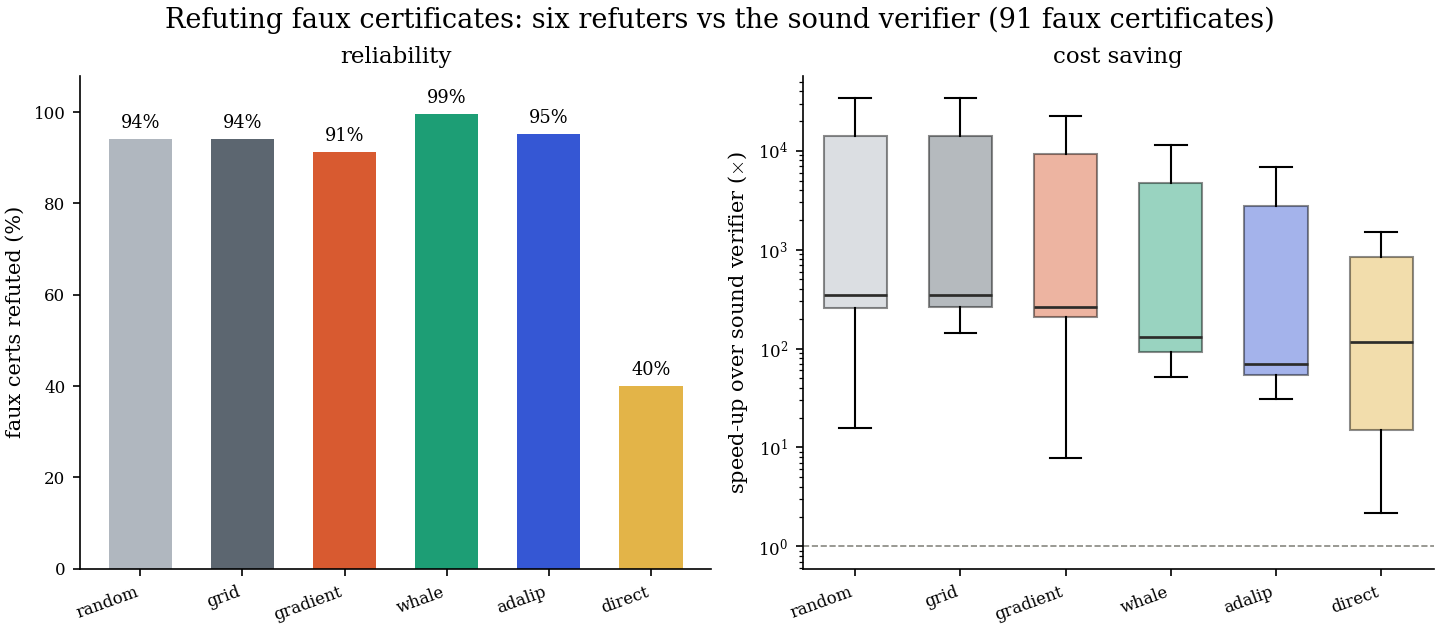
\includegraphics[width=\linewidth]{Figures/faux_certs.png}
\caption{Refuting the faux certificates a sound verifier rejected, six refuters
compared. \emph{Left:} the fraction of faux certificates each refuter refutes ---
whale is near-perfect, the other informed and uninformed methods cluster at
$91$--$95\%$, and DIRECT collapses to $40\%$. \emph{Right:} per-refuter speed-up
over the sound verifier (log): every refuter is one-to-three orders of magnitude
cheaper than a sound call, the fast uninformed searches highest.}
\label{fig:faux-certs}
\end{figure}

\begin{table}[t]
\centering
\begin{tabular}{lrrrrr}
\hline
Refuter & Success rate & Verifier (s) & Refuter (s) & Speed-up & Quality \\
\hline
Whale         & $99\%$ & $0.50$ & $0.004$ & $131\times$ & $0.049$ \\
AdaLIPO       & $95\%$ & $0.48$ & $0.007$ & $69\times$  & $0.042$ \\
Random        & $94\%$ & $0.48$ & $0.001$ & $344\times$ & $0.039$ \\
Grid          & $94\%$ & $0.48$ & $0.001$ & $352\times$ & $0.038$ \\
Hill climbing & $91\%$ & $0.48$ & $0.002$ & $262\times$ & $0.038$ \\
DIRECT        & $40\%$ & $0.48$ & $0.021$ & $116\times$ & $0.024$ \\
\hline
\end{tabular}
\caption{Faux-certificate refutation, six BBOB-tuned refuters versus the sound
verifier that rejected each candidate. Columns: the fraction of faux certificates
on which a genuine counterexample was found; \emph{median} wall-clock to a
counterexample for the verifier and the refuter, and their ratio; and median
counterexample quality (scored drift). Whale is the most reliable and returns the
deepest counterexamples; the uninformed searches are the cheapest per call;
DIRECT misses most of the linear-system certificates.}
\label{tab:fauxcert}
\end{table}


\newpage


